\section{Settings}


\begin{figure}[H]
	\centering
    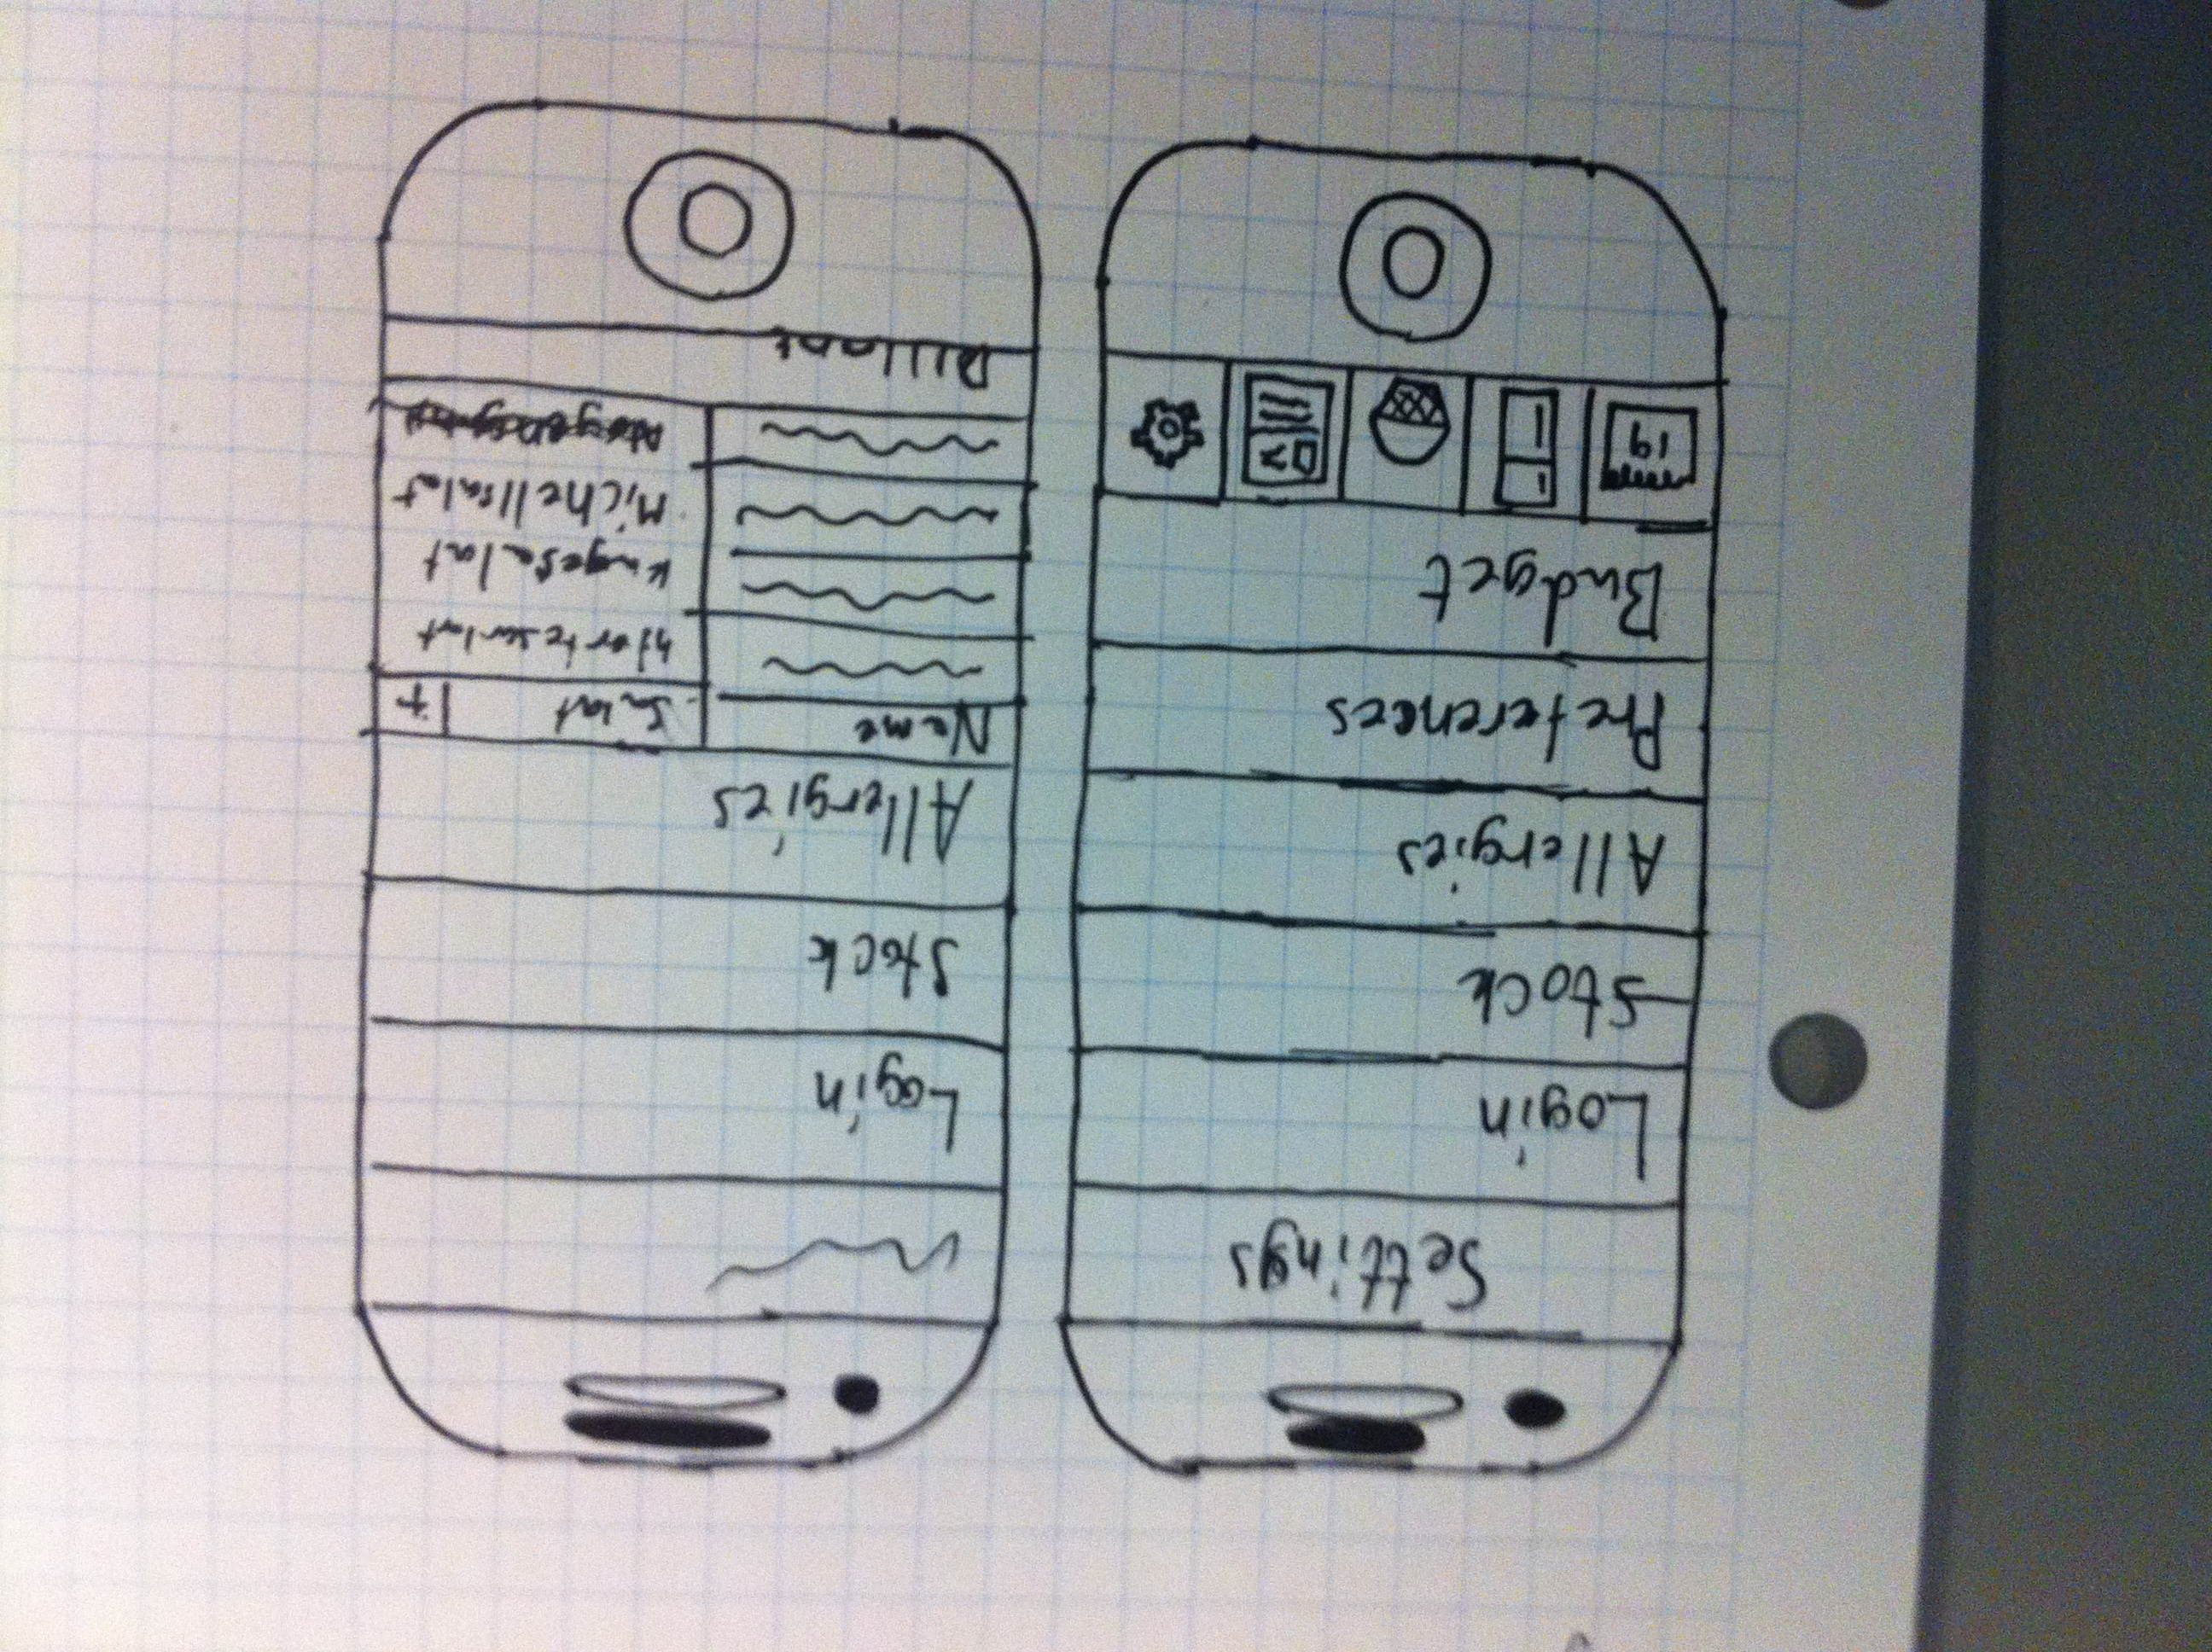
\includegraphics[width=0.5\textwidth]{Grafik/FoodPlanner/FinalSettingsSketch}
	\caption{This screen displays all of the settings in the program.}
	\label{SettingsScreen}
\end{figure}

The settings screen on \cref{SettingsScreen} has all the settings arranged as a list. To view details about a specific setting the user can press that setting and it will expand as the right screen on \cref{SettingsScreen}. The user will now have an overview of the specific information and options that is linked to the setting that has been selected.  